\documentclass[a4paper,ngerman]{article}

\usepackage[ngerman]{babel}
\usepackage[utf8]{inputenc}
\usepackage[
    pdftitle={DiVe - Distance Vector Routing Simulation},
	pdfauthor={Nico Kratky},
	pdfkeywords={distance vector, routing, networking, cpp}
]{hyperref}
\usepackage{fancyvrb}
\usepackage{minted}

\usepackage{graphicx}
\graphicspath{{images/}}

\usepackage[dvipsnames]{xcolor}
\definecolor{commentgreen}{RGB}{2,112,10}

\usepackage{listings}
\lstset{
language=C++,
numbers=left,
basicstyle=\ttfamily,
keywordstyle=\color{blue}\ttfamily,
stringstyle=\color{red}\ttfamily,
commentstyle=\color{commentgreen}\ttfamily,
aboveskip=1em,
belowskip=1em,
captionpos=b,
showstringspaces=false,
xleftmargin=2em,
framexleftmargin=1.5em
}

\usepackage{varioref}
\usepackage{parskip}

\usepackage[labelfont=bf]{caption}

\usepackage{placeins}

\title{%
    DiVe \\
    Distance Vector Routing Simulation
}
\author{Nico Kratky}

\begin{document}

\begin{titlepage}
\maketitle
\thispagestyle{empty}
\end{titlepage}

\tableofcontents
\clearpage

\section{Lizenz}
\begin{Verbatim}[fontsize=\small]
Boost Software License - Version 1.0 - August 17th, 2003

Permission is hereby granted, free of charge, to any person or organization
obtaining a copy of the software and accompanying documentation covered by
this license (the "Software") to use, reproduce, display, distribute,
execute, and transmit the Software, and to prepare derivative works of the
Software, and to permit third-parties to whom the Software is furnished to
do so, all subject to the following:

The copyright notices in the Software and this entire statement, including
the above license grant, this restriction and the following disclaimer,
must be included in all copies of the Software, in whole or in part, and
all derivative works of the Software, unless such copies or derivative
works are solely in the form of machine-executable object code generated by
a source language processor.

THE SOFTWARE IS PROVIDED "AS IS", WITHOUT WARRANTY OF ANY KIND, EXPRESS OR
IMPLIED, INCLUDING BUT NOT LIMITED TO THE WARRANTIES OF MERCHANTABILITY,
FITNESS FOR A PARTICULAR PURPOSE, TITLE AND NON-INFRINGEMENT. IN NO EVENT
SHALL THE COPYRIGHT HOLDERS OR ANYONE DISTRIBUTING THE SOFTWARE BE LIABLE
FOR ANY DAMAGES OR OTHER LIABILITY, WHETHER IN CONTRACT, TORT OR OTHERWISE,
ARISING FROM, OUT OF OR IN CONNECTION WITH THE SOFTWARE OR THE USE OR OTHER
DEALINGS IN THE SOFTWARE.

My apologies. When the previous paragraph was written, lowercase had not yet
been invented (that would involve another several millennia of evolution).
I did not mean to shout.
\end{Verbatim}
\clearpage

\section{Aufgabenstellung}

Die Aufgabe bestand darin, ein C++-Programm zur Simulation des Distanzvektor-Algorithmus zu entwickeln. Zusätzlich zum Algorithmus sollen zufällige Ausfälle der Verbindungen simuliert werden können.

\subsection{Verwendete Technologien}

Die zu verwendenden Technologien wurden vorgegeben. Nur Google Protocol Buffers wurden zusätzlich verwendet.

\begin{itemize}
    \item C++14
    \item CMake und make
    \item \{fmt\}
    \item spdlog
    \item JSON for Modern C++
    \item Asio (standalone Variante)
    \item Google Protocol Buffers
\end{itemize}

\subsection{Distanzvektor-Algorithmus}

Der Distanzvektor-Algorithmus ist eines der einfacheren Routing Protokolle. Es handelt nach dem Prinzip "Teile deinen Nachbarn mit, wie du die Welt siehst". Am Anfang kennt jeder Router nur seine Nachbarn und die Kosten dort hin. Dadurch, dass jeder Router seinen Nachbarn diesen sogenannten \textit{Distanzvektor} schickt, können nach einigen Iterationen die Wege zu den anderen Routern in der Topologie berechnet werden.

\section{Konzeption}

Für die Implementation der Simulation wurde nur ein einziges Programm entwickelt, dass einen Router repräsentieren soll. Dieses Programm baut durch mehrmaliges Starten mithilfe einer Konfigurationsdatei die gewünschte Netzwerktopologie auf. Das kann entweder auf ein und demselben Rechner geschehen oder auch verteilt über mehrere Hosts.

\subsection{Klassenstruktur}

Wie in Abbildung \vref{fig:uml} ersichtlich, verwaltet jeder Router jeweils eine Instanz der in Abschnitt \vref{sec:networking} beschriebenen Netzwerkkomponenten.

\begin{figure}[H]
    \centering
    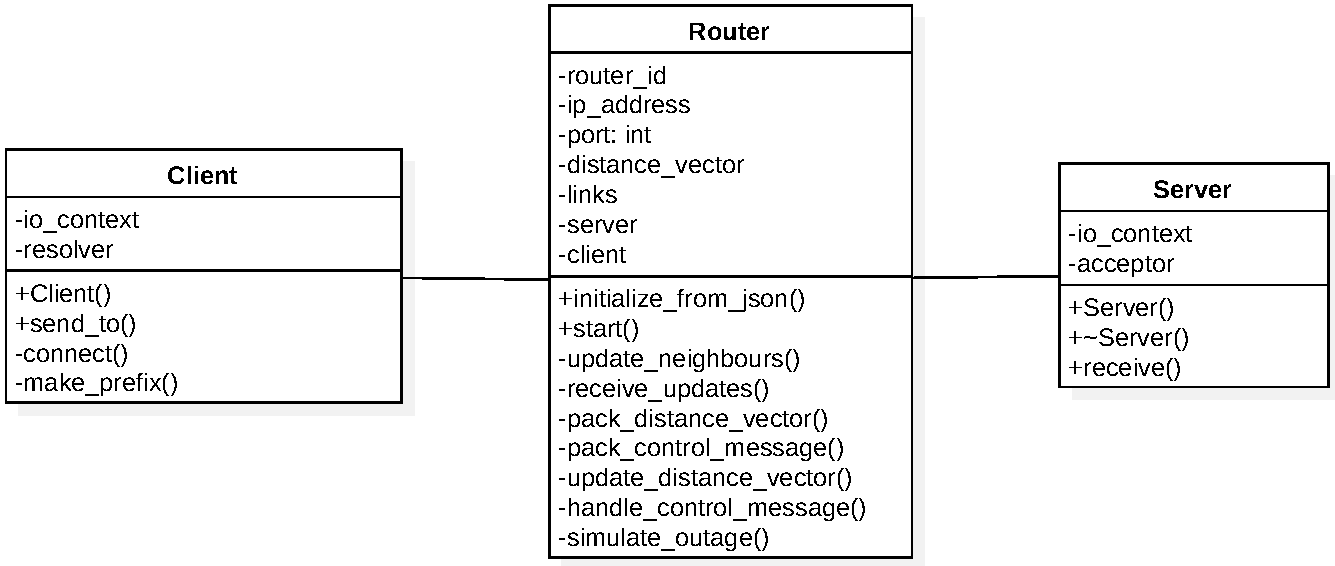
\includegraphics[width=\textwidth,keepaspectratio]{uml}
    \caption{UML Klassendiagramm}
    \label{fig:uml}
\end{figure}

\subsection{Programmablauf}

Zu Programmanfang parsed zunächst jeder Prozess die übergebene Konfigurationsdatei und baut den initialen Distanzvektor auf. Knoten, die laut Distanzvektor-Algorithmus mit $ \infty $ initialisiert werden müssten, werden mit $ -1 $ initialisiert, da der C++ Datentyp \lstinline{integer} keine Unendlichkeit kennt.  Dann beginnt eine Schleife die im angegebenen Intervall Routing Updates an seine Nachbarn schickt. Wenn ein Router so eine Nachricht erhält, beginnt er die empfangenen Kosten mit seinen Eigenen zu Vergleichen. Wenn die empfangenen Kosten, addiert mit den Kosten zu dem Router von dem das Update erhalten wurde, kleiner sind als die eigenen, trägt der Router diese Kosten in seinen eigenen Distanzvektor ein. Auch merkt er sich, dass dieser Router über den Router zu erreichen ist, von dem das Update gekommen ist.

\section{Konfiguration der Topologie}
\label{sec:configuration}

Die Netzwerktopologie kann durch eine JSON Konfigurationsdatei festgelegt werden. Eine Beispielkonfigurationsdatei ist im Appendix \vref{appendix:config} zu finden. Diese definiert eine Netzwerktopologie wie sie Abbildung \vref{fig:topology} zeigt.

\begin{figure}[H]
    \centering
    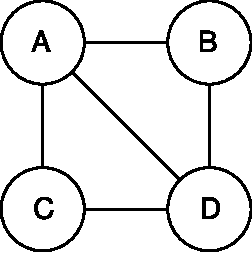
\includegraphics[width=3cm,keepaspectratio]{topology2}
    \caption{Darstellung der durch die in Appendix \vref{appendix:config} angeführte Datei konfigurierten Topologie}
    \label{fig:topology}
\end{figure}

Die Datei besteht aus einem \lstinline{nodes} Objekt und einem \lstinline{link} Array. \lstinline{nodes} enthält wiederum soviel Objekte wie es Router im Netzwerk gibt. Jedes Objekt benötigt ein \lstinline{ip_address} und \lstinline{port} Feld, damit der Prozess seine Netzwerkinformation und die der anderen Routern kennt. Das \lstinline{links} Array definiert wie die verschiedenen Router miteinander verbunden sind. Dazu wird einfach ein Objekt mit jeweils \lstinline{source} und \lstinline{target} und den Router IDs hinzugefügt. Die Reihenfolge zwischen den Elementen macht hierbei nur einen Unterschied, falls ein \textit{pof} Wert gesetzt ist. \textit{pof} steht hierbei für \textit{probability of failure}, was soviel bedeutet wie Ausfallwahrscheinlichkeit (siehe Abschnitt \vref{sec:outage_simulation}). Dieser Wert muss zwischen 0 und 1 liegen und gibt diese Wahrscheinlichkeit des Ausfalls der Verbindung von \textit{source} nach \textit{target} in Prozent an. Der Unterschied ist jedoch nicht für den Nutzer sichtbar. Er besteht lediglich in der Implementierung, da nur der \textit{source} Knoten berechnet ob ein Ausfall vorliegt und falls dies der Fall ist es an den \textit{target} Knoten weitergibt.

\section{Kommandozeile}

Als Benutzerschnittstelle werden Kommandozeilenparameter verwendet. Es gibt zwei Parameter die zwingend übergeben werden müssen. Dies sind einerseits die JSON Konfigurationsdatei und andererseits die Router ID. Die Router ID bestimmt welchen Router der eben gestartete Prozess in der konfigurierten Topologie widerspiegelt. Das Interval in dem die Routing Updates gesendet werden, kann durch den \textit{-i} bzw. \textit{--interval} eingestellt werden. Hier muss ein ganzzahliger Wert übergeben werden. Voreingestellt sind 5 Sekunden. Wenn der \textit{-v} bzw. \textit{--verbose} Parameter übergeben wird, dann werden zusätzliche Information ausgegeben.

\begin{listing}
\begin{minted}{bash}

SYNOPSIS
        ./router <topology file> <router id> [-i <seconds>] [-v]

OPTIONS
        -i, --interval
                    router update interval (default: 5)

        -v, --verbose
                    print additional debug information
\end{minted}
\end{listing}

\section{Netzwerkübertragung}
\label{sec:networking}

Für sämtliche Kommunikation zwischen Routern wird die C++ Bibliothek Asio verwendet. Zusätzlich werden zur Datenserialisierung Google Protocol Buffers eingesetzt.

Eine Besonderheit stellt die Tatsache, dass jeder Router Client und Server \textit{gleichzeitig} ist, dar.

Da laut Aufgabenbeschreibung TCP als Netzwerkprotokoll verwendet werden muss, wird zusätzlich zu jeder Nachricht ein Header mitgeschickt. Dieser Header enthält ausschließlich Informationen über die Länge des folgenden Datenpaketes. Dies geschieht, da TCP mit Datenströmen arbeitet und somit keine Information über Nachrichtengrenzen vorliegen. In diesem Projekt wird ein 4-Byte langes Feld in Network-byte Order verwendet, um diesen Header darzustellen.

Allerdings bildet diese Vorgehensweise ein Sicherheitsrisiko, da der empfangende Kommunikationspartner solange vom Datenstream liest, bis er die korrekte Anzahl an Bytes erreicht hat. Dies kann sich ein Angreifer zunutze machen und einen sehr großen Längen-Header in den Strom schicken. Die andere Seite wird nun sehr, sehr lange versuchen zu lesen.

\subsection{Verbindungsverwaltung}

Da ein Router zu sehr vielen Nachbarroutern verbunden sein könnte, und dies zu einem hohen Verwaltungsaufwand führen würde, wurde eine Implementierungsvariante ähnlich der von HTTP/1.0 gewählt. Dies bedeutet, dass für jeden Versand einer Nachricht eine eigene Verbindung zum Empfänger aufgebaut werden muss.

Dies hat sowohl Vorteile als auch Nachteile. Der große Vorteil besteht darin, dass die Router die offenen Verbindungen nicht verwalten müssen. Der Nachteil besteht darin, dass diese Vorgehensweise höhere Netzwerkbelastung verursacht und auch mehr Rechenleistung der beiden Router verlangt. Diese beiden Nachteile können in der heutigen Zeit jedoch vernachlässigt werden, da diese Belastungen so minimal sind, dass sie praktisch keinen Unterschied machen. Der einzige wirkliche Nachteil ist ein höherer Implementierungsaufwand bezüglich der Ausfallsimulation, da ein Ausfall nicht einfach durch ein Schließen einer Verbindung simuliert werden kann.

Die beiden Begriffe \textit{Server} und \textit{Client} sind in diesem Projekt gleichzusetzen mit Empfänger und Sender, da die beiden Komponenten nichts anderes machen außer eben empfangen und senden.

\subsection{Server}

Wie schon eben erwähnt, dient der Server nur dazu, um Nachrichten von anderen Routern zu empfangen. Dies passiert dadurch, dass beim Start des Routers ein Thread erzeugt wird, der in einer Endlosschleife Nachrichten empfängt und sie an die entsprechenden Funktionen zur weiteren Behandlung weitergibt. Codebeispiel \vref{code:router_receive} zeigt die Methode die diese eben genannte Funktionalität implementiert.

\begin{listing}
\begin{minted}{cpp}
for (;;) {
    logger_->info("waiting for update");
    dive::Message update{server_.receive()};

    if (update.has_dv()) {
        update_distance_vector(update.dv());
    } else if (update.has_cm()) {
        handle_control_message(update.cm());
    }
}
\end{minted}

\caption{Methode der Klasse Router zum Empfangen eventuell ankommender Nachrichten. Wird als Thread gestarted.}
\label{code:router_receive}
\end{listing}

\FloatBarrier
\subsection{Client}

Ähnlich zum Server ist der Client nur für das Senden von Nachrichten zuständig. Wenn die \textit{send\_to} Methode aufgerufen wird, baut der Client zunächst eine Verbindung zum Server auf. Da die Methode bereits ein serialisiertes Objekt als Parameter bekommet, muss nur noch die Länge berechnet, und in Network-byte Order umgewandelt werden. Diese beiden Nachrichtenteile werden dann an den Server versandt. Codebeispiel \vref{code:client_send} zeigt den wichtigsten Ausschnitt dieser Methode.

\begin{listing}
\begin{minted}{cpp}
connect(sock, endpoints);

uint32_t prefix{make_prefix(message)};

logger_->trace("Message prefix: {}", prefix);

asio::error_code ec;

std::size_t sent{0};

sent += asio::write(sock, asio::buffer(&prefix,
                                       sizeof(prefix)),
                    ec);
sent += asio::write(sock, asio::buffer(message), ec);

logger_->info("Message sent");

sock.close();
\end{minted}

\caption{Ausschnitt aus der send\_to Methode der Klasse Client}
\label{code:client_send}
\end{listing}

\subsection{Nachrichtentypen}

In diesem Projekt wurden zwei verschiedene Nachrichtentypen verwendet. Einerseits die normalen Routingupdates und andererseits sogenannte \textit{Control Messages}. Diese dienen ganz einfach dazu, dem Empfänger ein Kommando zu schicken.

Jedes Protobuf Objekt hat ein Feld \lstinline{router_id}, das die Router ID des Absender enthält. Dieses dient dazu um die Nachrichten schneller den Routern zuordnen zu können.

Codebeispiel \vref{code:protobuf} zeigt die verwendeten Protobuf Nachrichten.

\begin{listing}
\begin{minted}{protobuf}
syntax = "proto3";

package dive;

message DistanceVector {
    string router_id = 1;

    message Distance {
        string router_id = 1;
        sint32 distance = 2;
    }

    repeated Distance distance_vector = 2;
}

message ControlMessage {
    string router_id = 1;

    string data = 2;
}

message Message {
    oneof Data {
        DistanceVector dv = 1;
        ControlMessage cm = 2;
    }
}
\end{minted}

\caption{Protobuf}
\label{code:protobuf}
\end{listing}

\section{Ausfallsimulation}
\label{sec:outage_simulation}

Der zufällige Ausfall von Verbindungen zwischen jeweils zwei Routern kann durch zusätzliche Konfiguration simuliert werden. Da der Distanzvektor-Algorithmus solche Ausfälle automatisch erkennt und seine Routingtabelle dementsprechend aktualisiert, ist er in die Gruppe der \textit{dynamischen} Routingprotokolle einzuordnen.

Wie schon in Abschnitt \vref{sec:configuration} erwähnt, erfolgt solch eine Ausfallsimulation durch hinzufügen eines \textit{pof} Wertes in die Konfigurationsdatei.

Implementiert ist diese Simulation als Bernoulli-Verteilung. Diese Verteilung hat nur zwei mögliche Resultate, entweder 0 oder 1, was in diesem Fall einem Wahrheitswert entspricht und das Zustandekommen einer Ausfallsimulation bestimmt. Bei der Instanzierung wird die Wahrscheinlichkeit eines positiven Ausgangs mitgegeben und danach wie eine Funktion aufgerufen. Diese gibt dann \lstinline{true} oder \lstinline{false} zurück.

\begin{listing}
\begin{minted}{cpp}
void Router::simulate_outage() {
    std::random_device rd;
    std::mt19937 gen{rd()};

    std::bernoulli_distribution d{pof_};

    if(d(gen)) {
        // Verbindung soll ausfallen
    } else {
        // Kein Ausfall
    }
}
\end{minted}

\caption{Ausfallsimulation}
\label{code:simulate_outage}
\end{listing}


Wenn ein Router mithilfe dieser Methode feststellt, dass eine Verbindung ausgefallen ist, setzt er die Kosten zu dem Router auf der anderen Seite dieser Verbindung auf $ \infty $. Anschließend sendet er eine \lstinline{Control Message} an den Router auf der anderen Seite, um ihm mitzuteilen, dass diese Verbindung ausgefallen ist. Alle anderen Routern erfahren dies über die Routing Updates.

\section{Dokumentation}

Der Code des Projekts wurde in einem Doxygen-konformen Stil dokumentiert. Mithilfe von Doxygen können dann aus diesen Kommentaren übersichtliche Dokumentationen in Formaten wie PDF oder \LaTeX\ generiert werden. Codebeispiel \vref{code:doxygen} zeigt die notwendigen Schritte um diese Dokumentation zu generieren. Einzige Vorraussetzung dafür ist, dass Doxygen korrekt installiert ist.

\begin{listing}
\begin{minted}{bash}
cd build
cmake .. -DBUILD_DOC=ON
make doc
\end{minted}

\caption{Generierung von Dokumentation mithilfe von Doxygen}
\label{code:doxygen}
\end{listing}

Nach diesen Schritten ist im Verzeichnis \lstinline{doc} die Dokumentation als PDF und \LaTeX\ zu finden.

\clearpage
\begin{appendix}

\section{Beispielkonfigurationsdatei}
\label{appendix:config}

\begin{minted}{json}
{
    "nodes": {
        "A": {
            "ip_address": "127.0.0.1",
            "port": 16022
        },
        "B": {
            "ip_address": "127.0.0.1",
            "port": 16023
        },
        "C": {
            "ip_address": "127.0.0.1",
            "port": 16024
        },
        "D": {
            "ip_address": "127.0.0.1",
            "port": 16025
        }
    },
    "links": [
        {
            "source": "A",
            "target": "D"
        },
        {
            "source": "A",
            "target": "B"
        },
        {
            "source": "A",
            "target": "C"
        },
        {
            "source": "B",
            "target": "D"
        },
        {
            "source": "C",
            "target": "D"
        }
        ]
}
\end{minted}

\end{appendix}

\end{document}
